% \chapter{Design and Implementation}
\chapter{Alg: Algebraic Functional Language}
Algebraic Functional Language (Alg) is an example of the high-level languages to generate parallel code, proposed in the paper \cite{AlgebraicMultipartyProtocol}. The work done by \cite{AlgebraicMultipartyProtocol} also proposes a method to do the code generation. Part of this project is about implementing an alternative code generation backend for the PAL. In the evaluation section, we will compare the speed of generated code of our method against the original method. We will give an overview of the language in this section.  
\section{Alg}
This section is an overview of Alg language. 
\subsection{Syntax}
Besides primitives type like int, unit and function types, Alg use four functors to form more types hence representing complicated data structures by composing them (seen in table). For example, a list of integer is expressed in \coref{p:pal:c1}.
\begin{table}[ht]
\begin{grammar}{F_1, F_2 \Coloneqq}{}
    I & Identity functor\\
    K t & Constatnt functor\\
    F_1 + F_2 & Sum functor\\
    F_1 \times F_2 & Product functor
\end{grammar}
\hfill
\begin{grammar}{t_1, t_2 \Coloneqq}{Type}
    () \mid \text{int} \mid \dots & Primitive types\\
    F \ t_1 & Functor types\\
    \mu .F & Recursive types\\
\end{grammar}
\caption{Functor and Type definitions}
\end{table}
\begin{code}
\begin{lstlisting}{language=Haskell}
    newtype L = K () + K Int * I
    type List = Rec L
\end{lstlisting}
\caption{Type of integer list in PAL}
\label{p:pal:c1}
\end{code}

An important feature of Alg is the lack of usual control flow like if branch or while loop, instead, it uses data structures to replace control flow. Data structures in PAL not only store data but also serves as control structures. It uses the idea of recursion schemes (seen in \secref{b:rs}) to build sophisticated algorithms. 

To summary, algorithms in Alg are represented as a series of transformations of data, making it easy to transform the Alg programs to programs in arrows mechanically since arrows also express flow of data and their transformations naturally. This property allows us to generate parallel code without burners.

\subsection{Example: Merge sort}

Like the merge sort example in \secref{b:rs:ex}, PAL make these recursion schemes built-in and hence express computation. A merge sort in PAL is shown in \coref{p:pal:c5}
\begin{listing}[ht]
\begin{lstlisting}[language=haskell]
poly T = K (() + int) + I * I;
poly L = K () + K int * I;

atom split : Rec L -> T Rec L;

atom merge : T Rec L -> Rec L;

fun ms : Rec L -> Rec L
  = rec [T] merge split;
\end{lstlisting}
\caption{Merge sort in Alg} \label{p:pal:c5}
\end{listing}
\section{ParAlg: Alg + role annotations}
\subsection{Inferring global types}
\subsection{Example: Parallel merge sort}
\section{Conclusion}
\begin{figure}[ht]
    \centering
    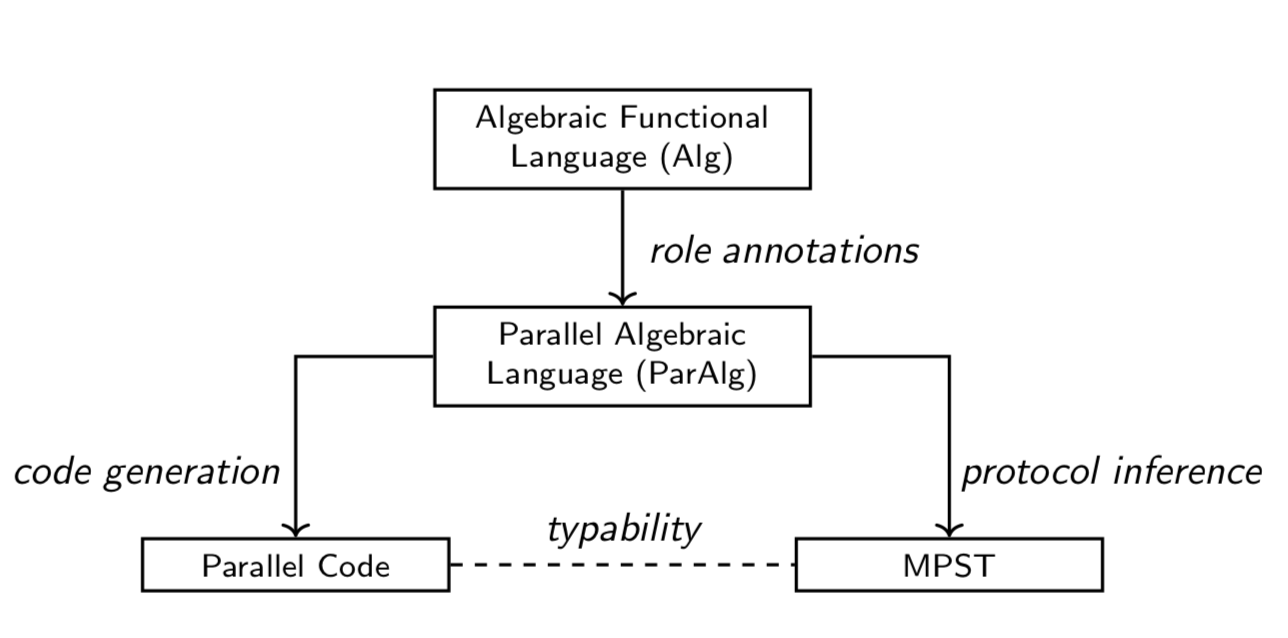
\includegraphics[width=0.7\textwidth]{project/pipeline.png}
    \caption{Overview of code generating pipeline from Alg\cite{AlgebraicMultipartyProtocol}}
    \label{project:fig:pipeline}
\end{figure}
A visualization of the pipeline can be seen in the \figref{project:fig:pipeline}. The content of the section is a skim of Alg and ParAlg. Curious readers should read about \cite{AlgebraicMultipartyProtocol} for more details.

Combinators and the syntax of Alg makes every Alg program to be point-free. Without the use of explicit variables, point-free programs express the underlying data-flow of the computation clearly. Adding role annotations transforms Alg programs to ParAlg programs converting the implicit data-flow to explicit communication. Communication will aid us generate parallel code using message-passing concurrency. We will introduce the our method from next chapter.  